%\documentstyle[epsf,twocolumn]{jarticle}       %LaTeX2.09仕様
%\documentclass[twocolumn]{jarticle}     %pLaTeX2e仕様
\documentclass{jarticle}     %pLaTeX2e仕様

%一枚組だったら[twocolumn]関係のとこ消す

\setlength{\topmargin}{-45pt}
%\setlength{\oddsidemargin}{0cm} 
\setlength{\oddsidemargin}{-7.5mm}
%\setlength{\evensidemargin}{0cm} 
\setlength{\textheight}{24.1cm}
%setlength{\textheight}{25cm} 
\setlength{\textwidth}{17.4cm}
%\setlength{\textwidth}{172mm} 
\setlength{\columnsep}{11mm}

\kanjiskip=.07zw plus.5pt minus.5pt

\usepackage[dvipdfm]{graphicx}
\usepackage{ccaption}
\usepackage{algorithm}
\usepackage{algorithmic}
\usepackage{subcaption}
\usepackage{enumerate}
\usepackage{comment}
\usepackage{url}
\usepackage{multirow}
\usepackage{diagbox}
\usepackage{amssymb}
\usepackage{mathtools}
\usepackage{wrapfig}
\usepackage{graphicx}
\usepackage{float}
\usepackage{amsmath}
\usepackage{lipsum}


\begin{document}
  \noindent
  \hspace{1em}

  \today Creation班 ゼミ
  \hfill
  \ \  西村昭賢 

  \vspace{2mm}
  \hrule
  \begin{center}
  {\Large \bf 進捗報告}
  \end{center}
  \hrule
  \vspace{3mm}


\section{やったこと}
3つの目的関数における多目的最適化GAの適用

\section{3目的のNSGA-II}
本実験では以下の3つの目的関数を用いた. 卒業研究では $f_\mathrm{w}$, $f_\mathrm{p}$で NSGA-II を適用し, 比較対象としていた.
\begin{itemize}
  \item 戦略間の勝率 $f_\mathrm{w}$
  \item カードのパラメータの変化量 $f_\mathrm{p}$
  \item 調整されるカードの種類数 $f_\mathrm{c}$
\end{itemize}

図 \ref{fig:result} に解空間における最終世代の個体群を示す. 
赤点がパレートフロント上の解, 青点がそれ以外の解を表している.

図 \ref{fig:fwfp_add}, \ref{fig:fwfp_noadd} に縦軸が $f_\mathrm{w}$, 横軸が $f_\mathrm{p}$ である散布図を示す.
また, 同様に図 \ref{fig:fwfc_noadd}, \ref{fig:fwfc_add} に縦軸が $f_\mathrm{w}$, 横軸が $f_\mathrm{c}$ である散布図を示す.
図の緑点, 赤点, 青点がそれぞれ卒業研究で用いた単目的 GA, 多目的 GA (2 目的の NSGA-II)の最終世代のパレートフロント, 提案手法の解群を表している.

\begin{figure}[ht]
  \centering
  \includegraphics[width=90mm]{assets/cardgameNSGA2.eps}
  \vspace{-0.3cm}
  \caption{最終世代の個体群の解空間のプロット}
  \label{fig:result}
\end{figure}

\begin{figure}[ht]
  \centering
  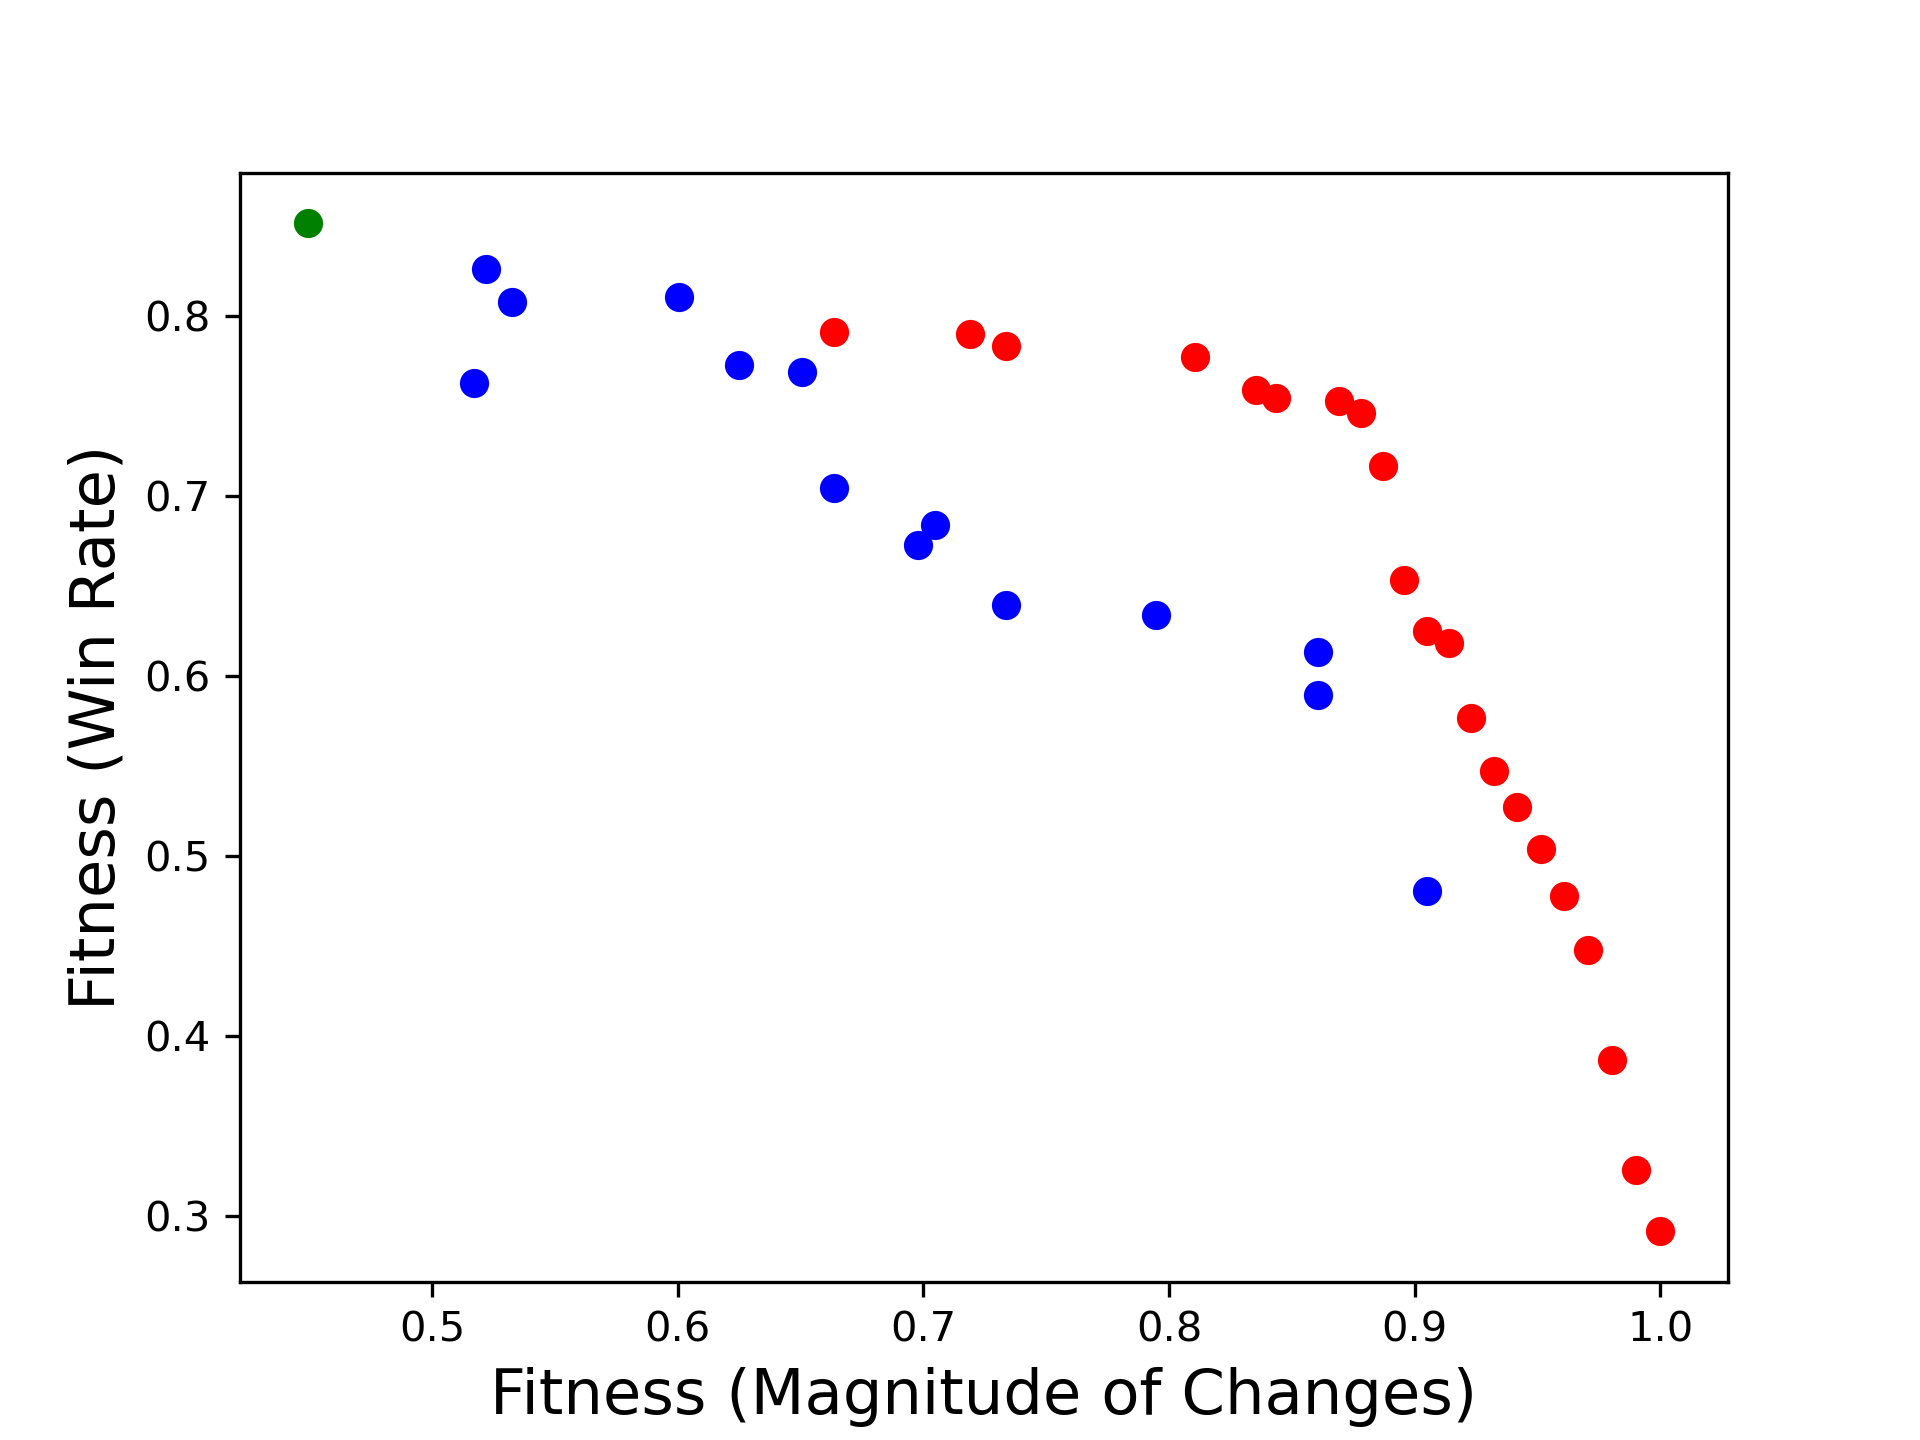
\includegraphics[width=120mm]{assets/fwfp_noadd.eps}
  \vspace{-0.3cm}
  \caption{最終世代の個体群の解空間のプロット}
  \label{fig:fwfp_noadd}
\end{figure}

\newpage

\begin{figure}[ht]
  \centering
  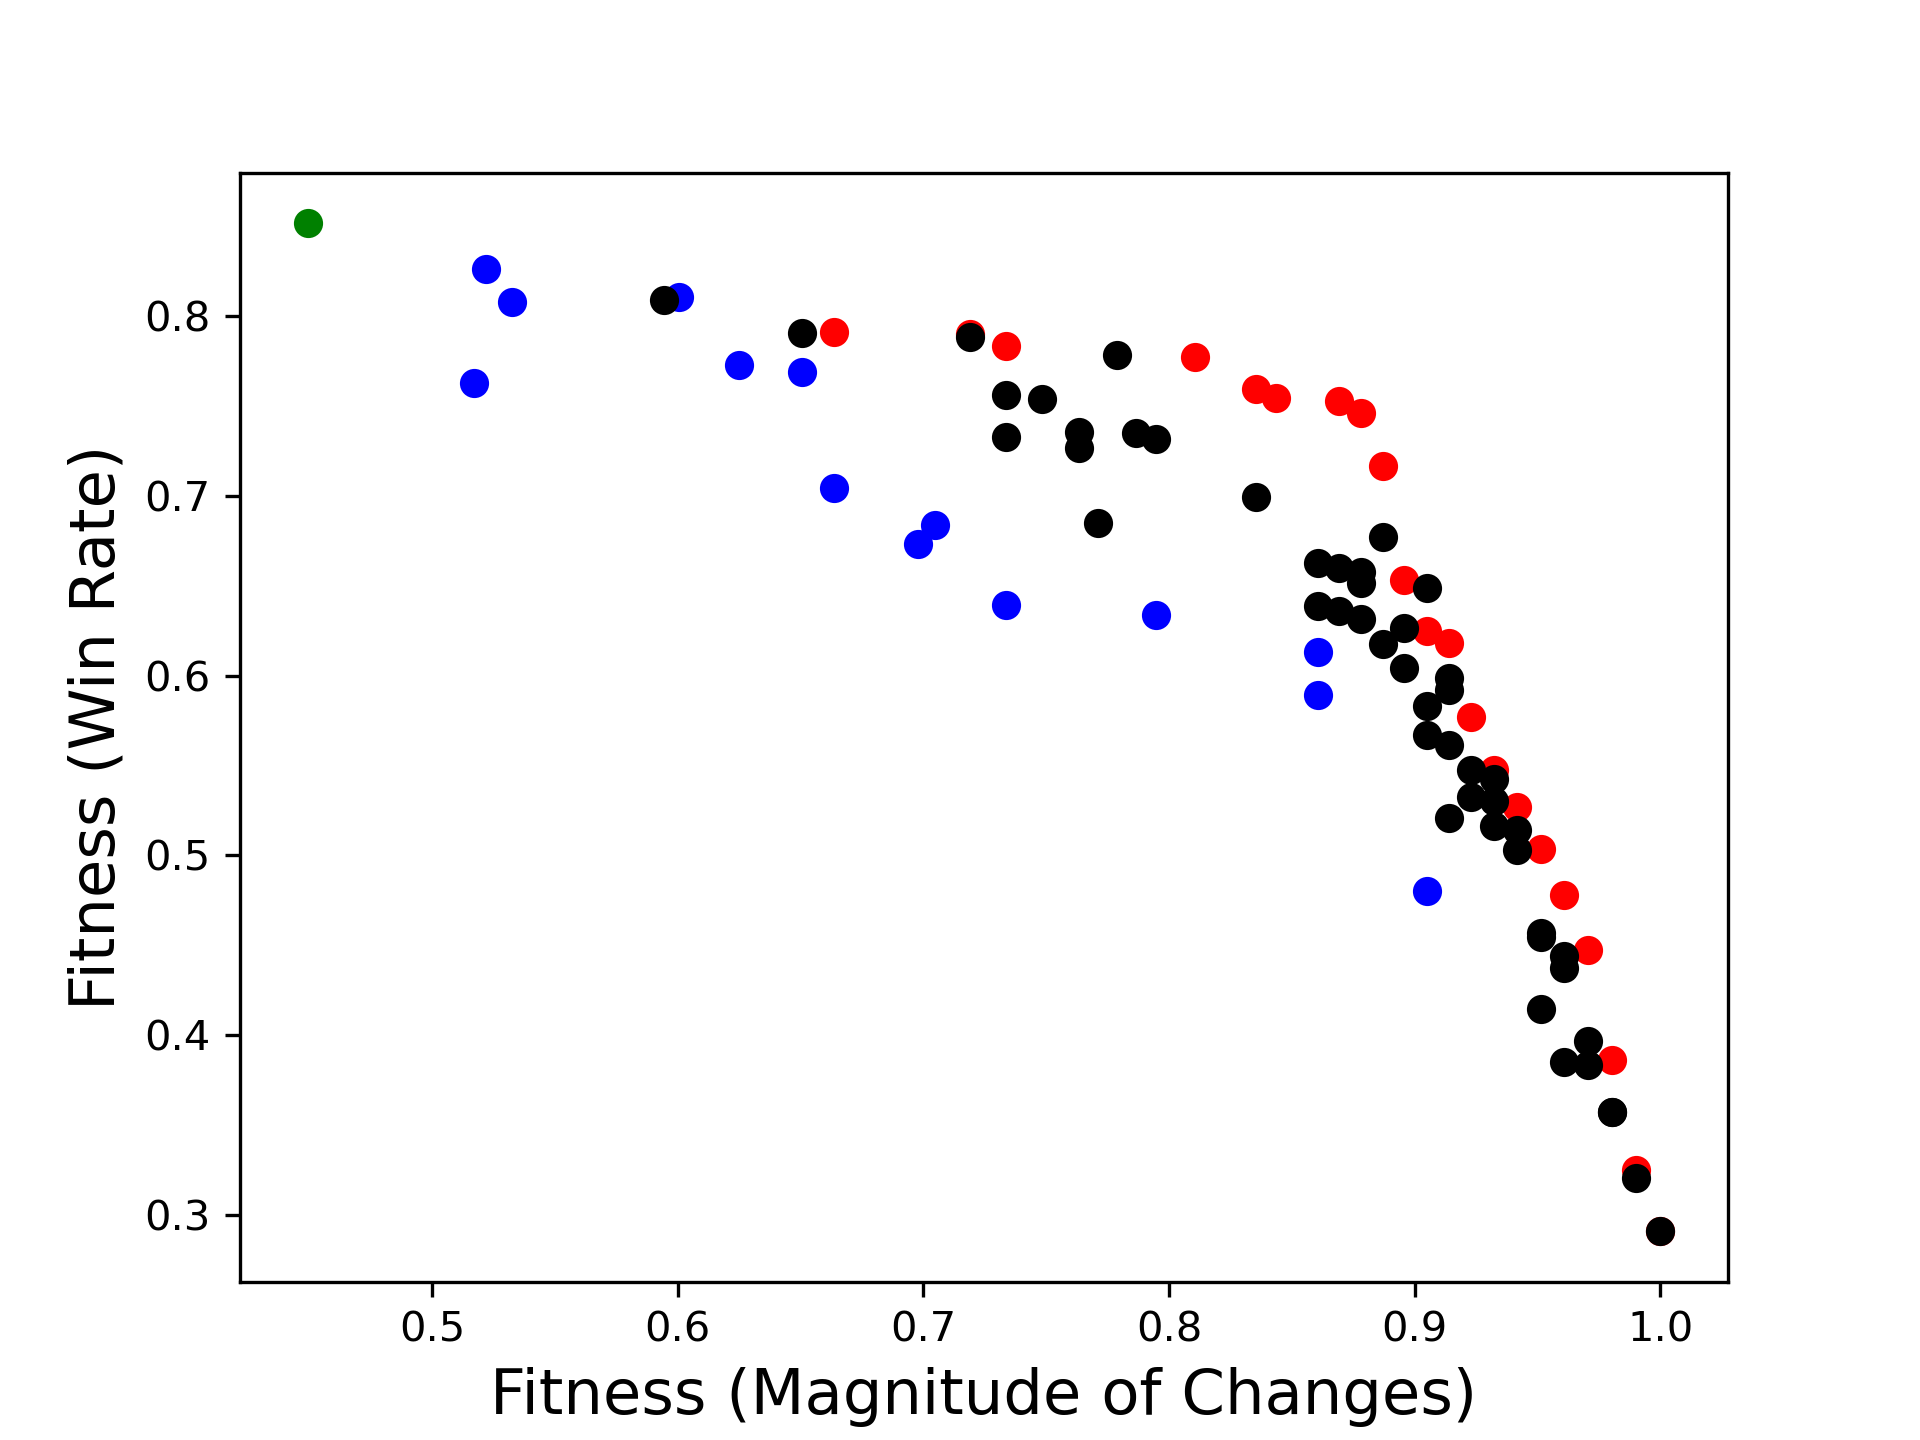
\includegraphics[width=120mm]{assets/fwfp_add.eps}
  \vspace{-0.3cm}
  \caption{最終世代の個体群の解空間のプロット}
  \label{fig:fwfp_add}
\end{figure}

\newpage 

\begin{figure}[ht]
  \centering
  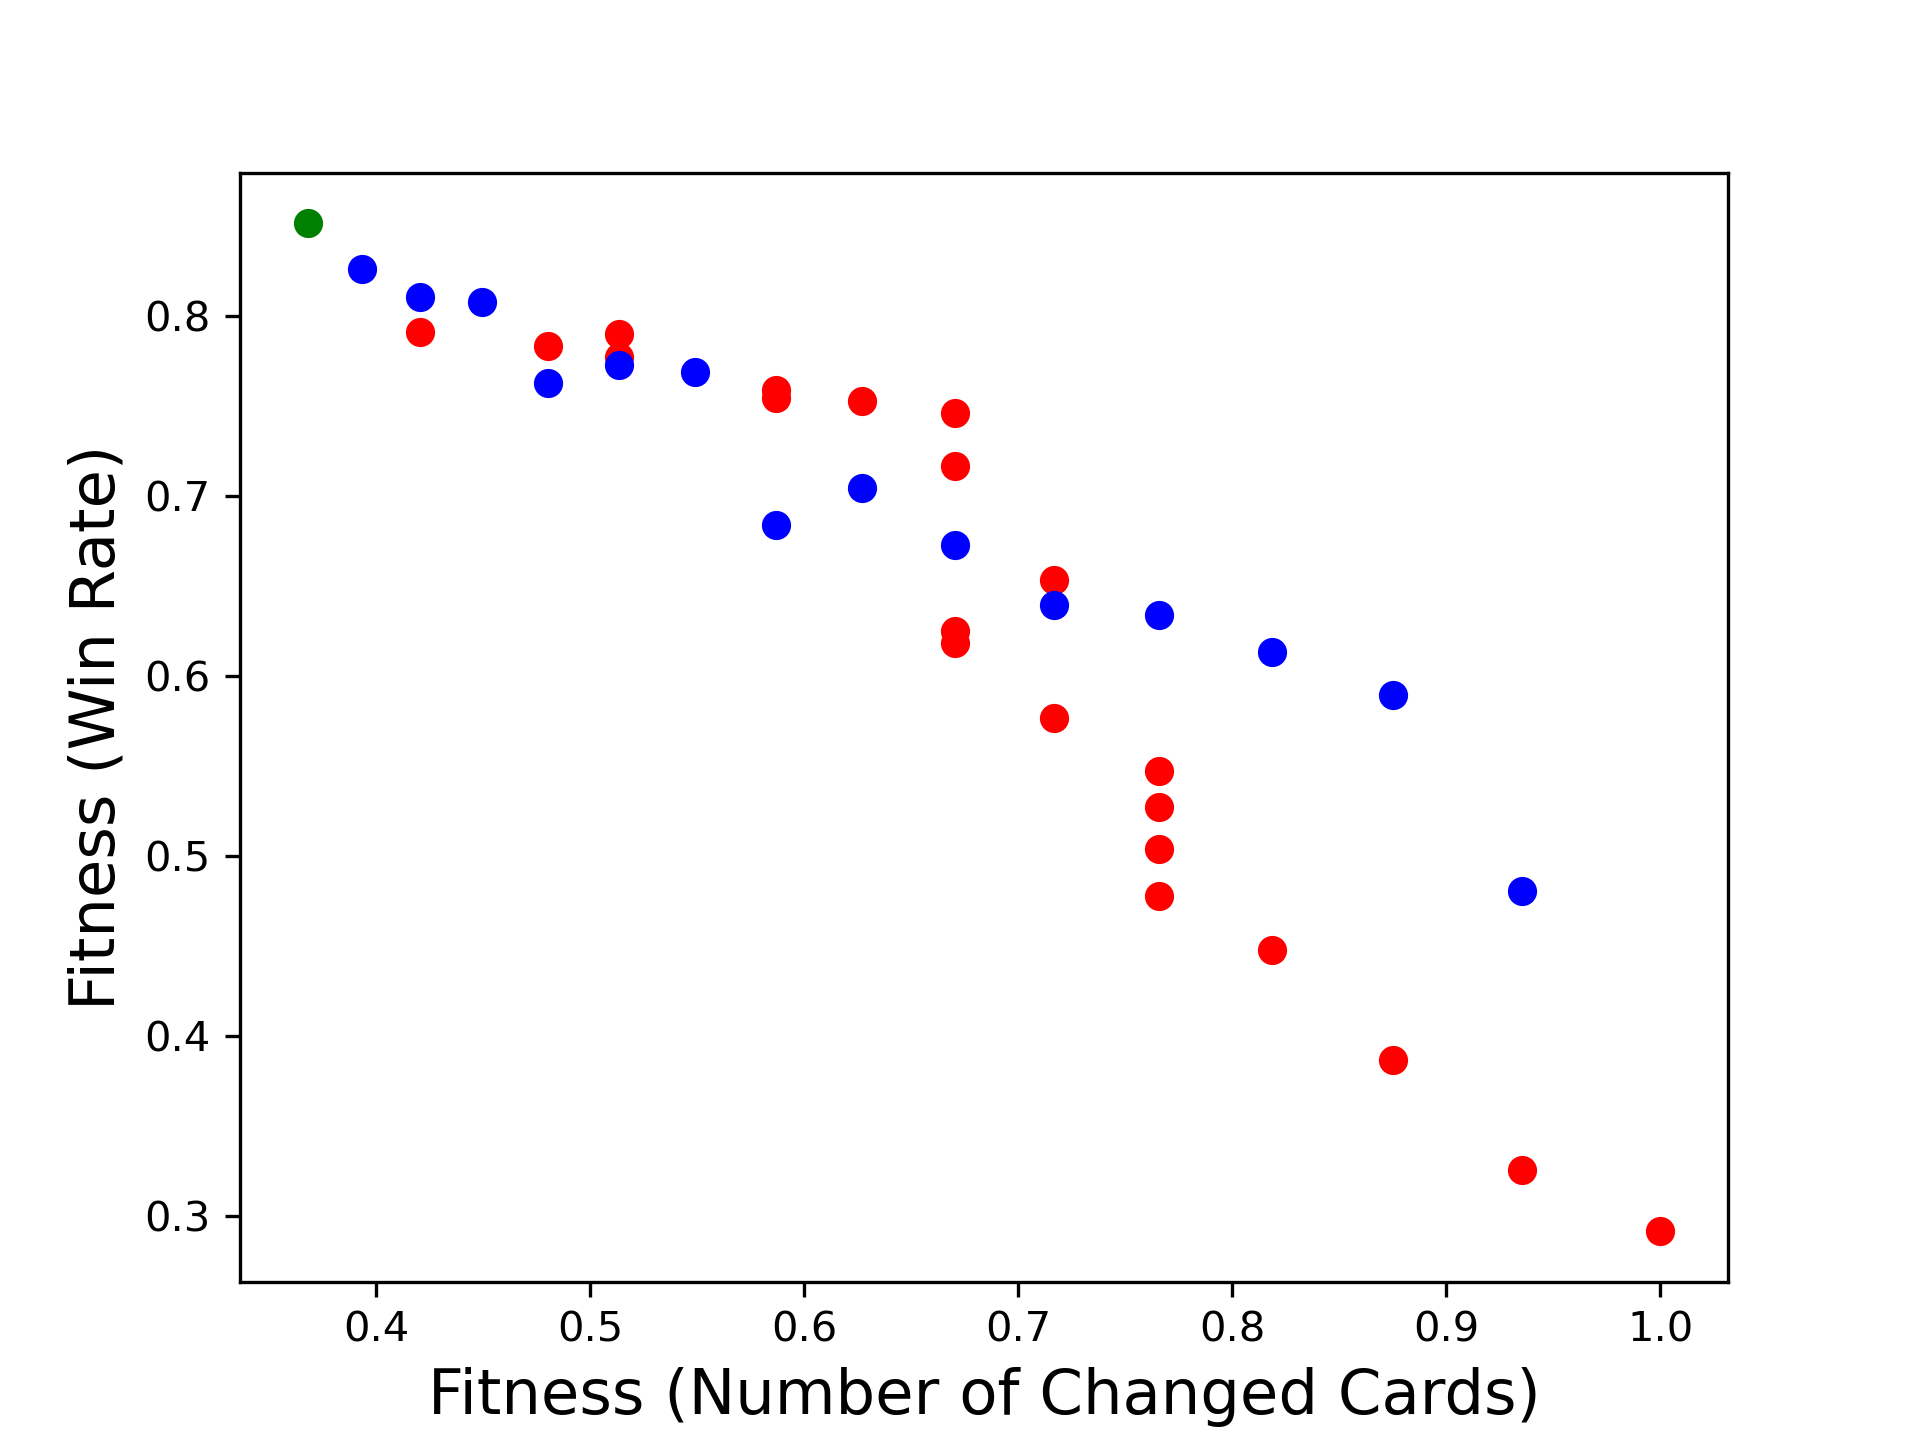
\includegraphics[width=120mm]{assets/fwfc_noadd.eps}
  \vspace{-0.3cm}
  \caption{最終世代の個体群の解空間のプロット}
  \label{fig:fwfc_noadd}
\end{figure}

\begin{figure}[ht]
  \centering
  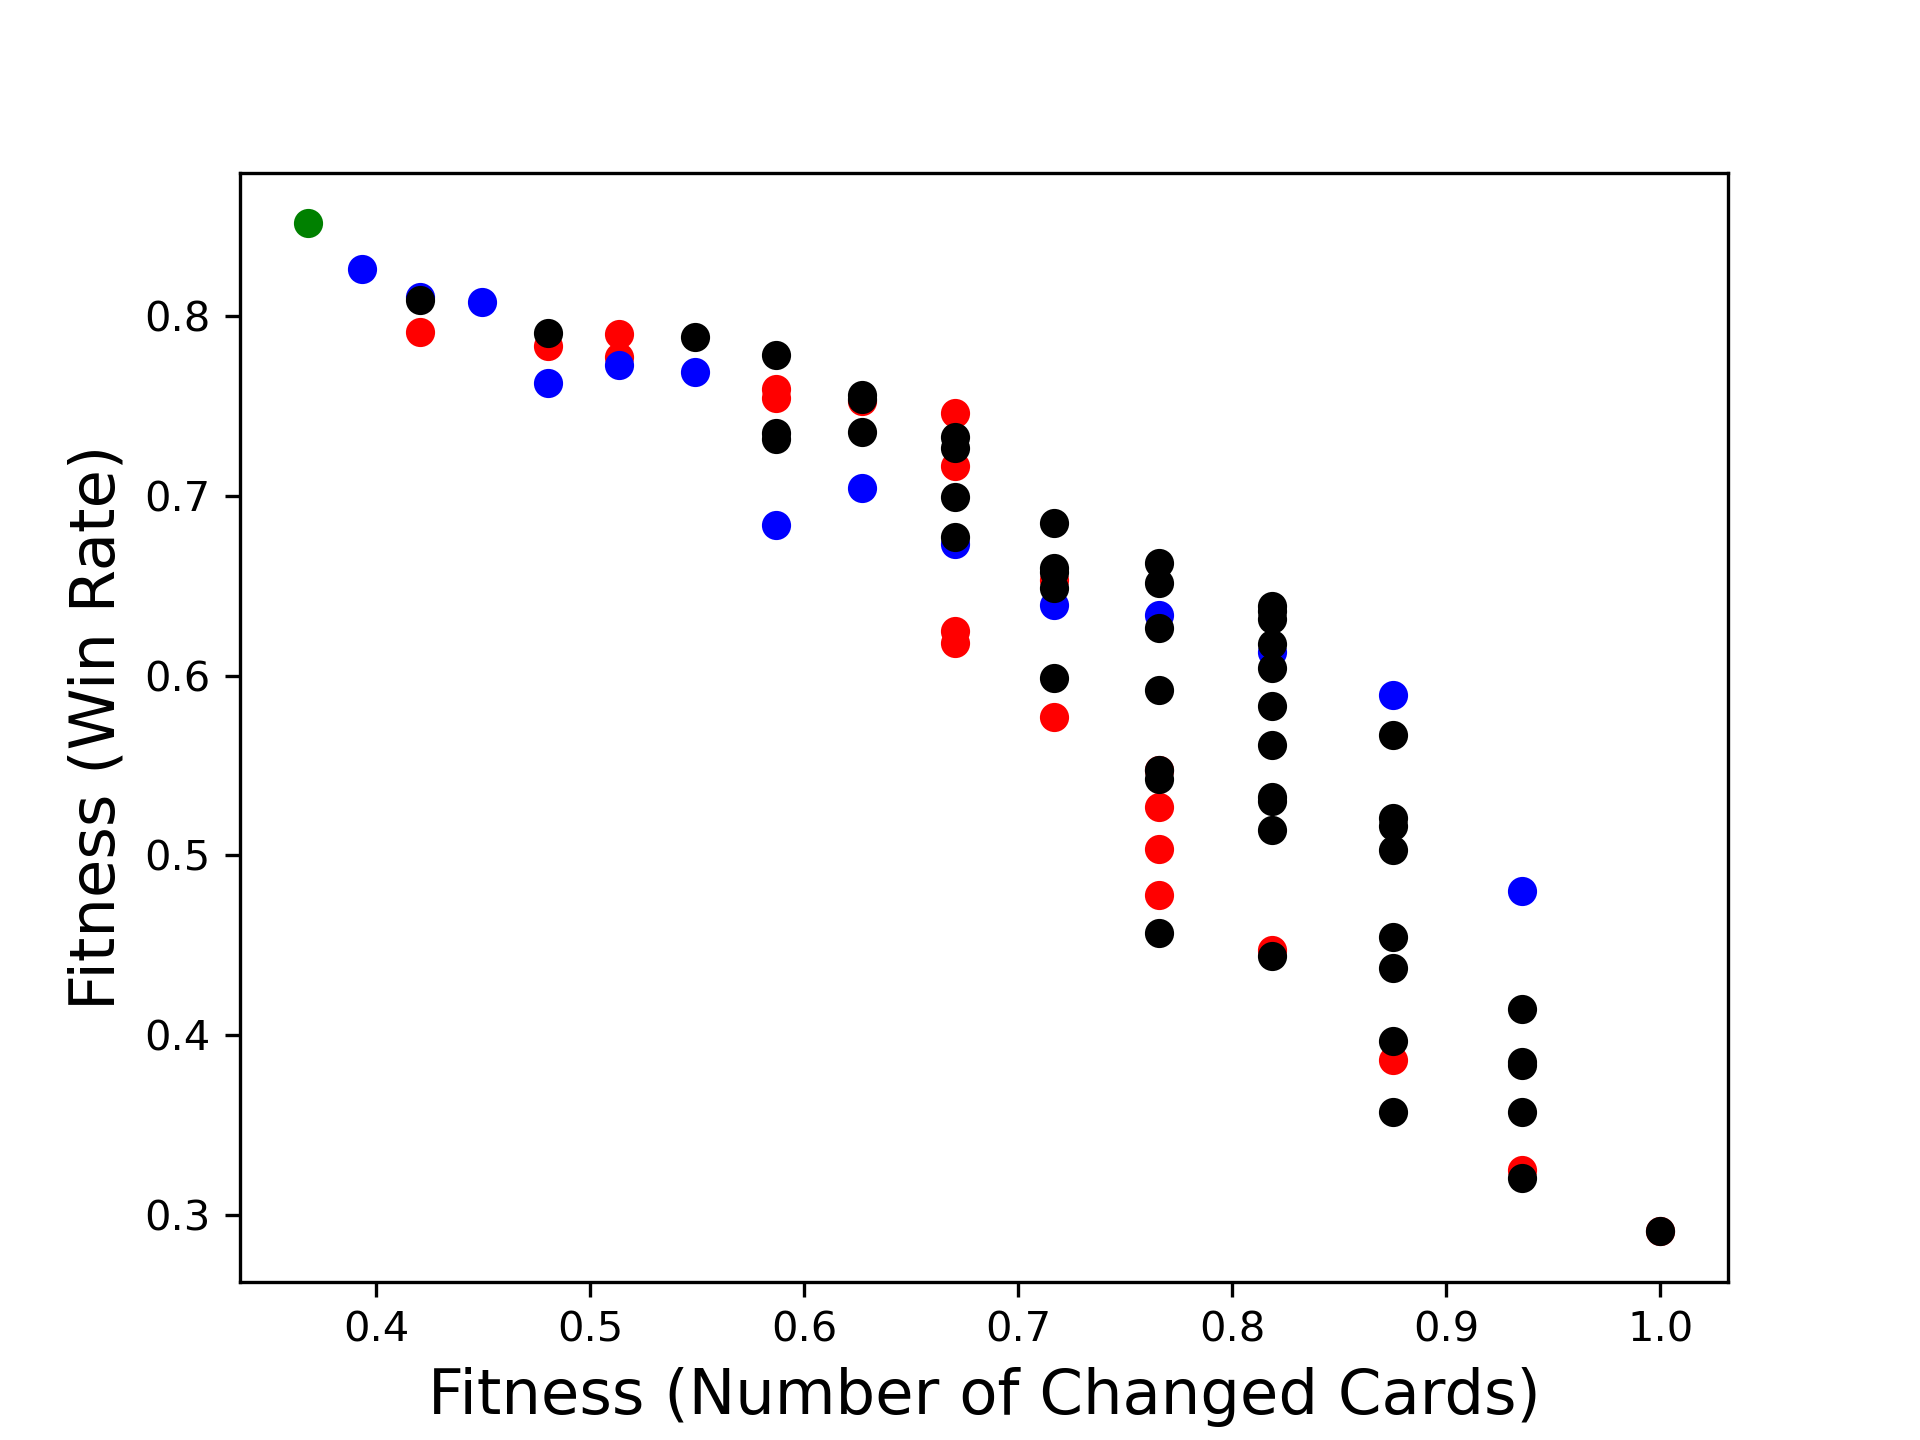
\includegraphics[width=120mm]{assets/fwfc_add.eps}
  \vspace{-0.3cm}
  \caption{最終世代の個体群の解空間のプロット}
  \label{fig:fwfc_add}
\end{figure}

$f_\mathrm{w}$ に関してのみ考えると, 単目的 GA と提案手法(予め調整する対象を限定して単目的 GA) が良好な解を作成できている. 
これは, 各手法について同世代数, 同個体数で実験を回しており、多目的GAでは $f_\mathrm{w}$ に関して良好ではない解が保存されるためこのような結果になったと考えられる. 
また, 図 \ref{fig:fwfc_add} に関して, 「調整するカード枚数を減らしながらデッキ間の勝率を最適化する」という目的では今回の 3 目的の GA で得られた解が多くの場合優れていることが分かった.


%index.bibはtexファイルと同階層に置く
%ちゃんと\citeしないと表示されない(1敗)
\bibliography{index.bib}
\bibliographystyle{junsrt}

\end{document}